%!TEX root = ../main.tex 

\section{Comment une impédance?}

\subsection{Matching à la source}

\begin{frame}{Matching à la source}
    \begin{itemize}
        \item Plupart des circuits avec sortie CMOS
        \item $Z_o \rightarrow 0\Omega$
    \end{itemize}
    \begin{columns}
        \begin{column}{0.25\textwidth}
            \begin{center}
                \begin{figure}
                \centering
                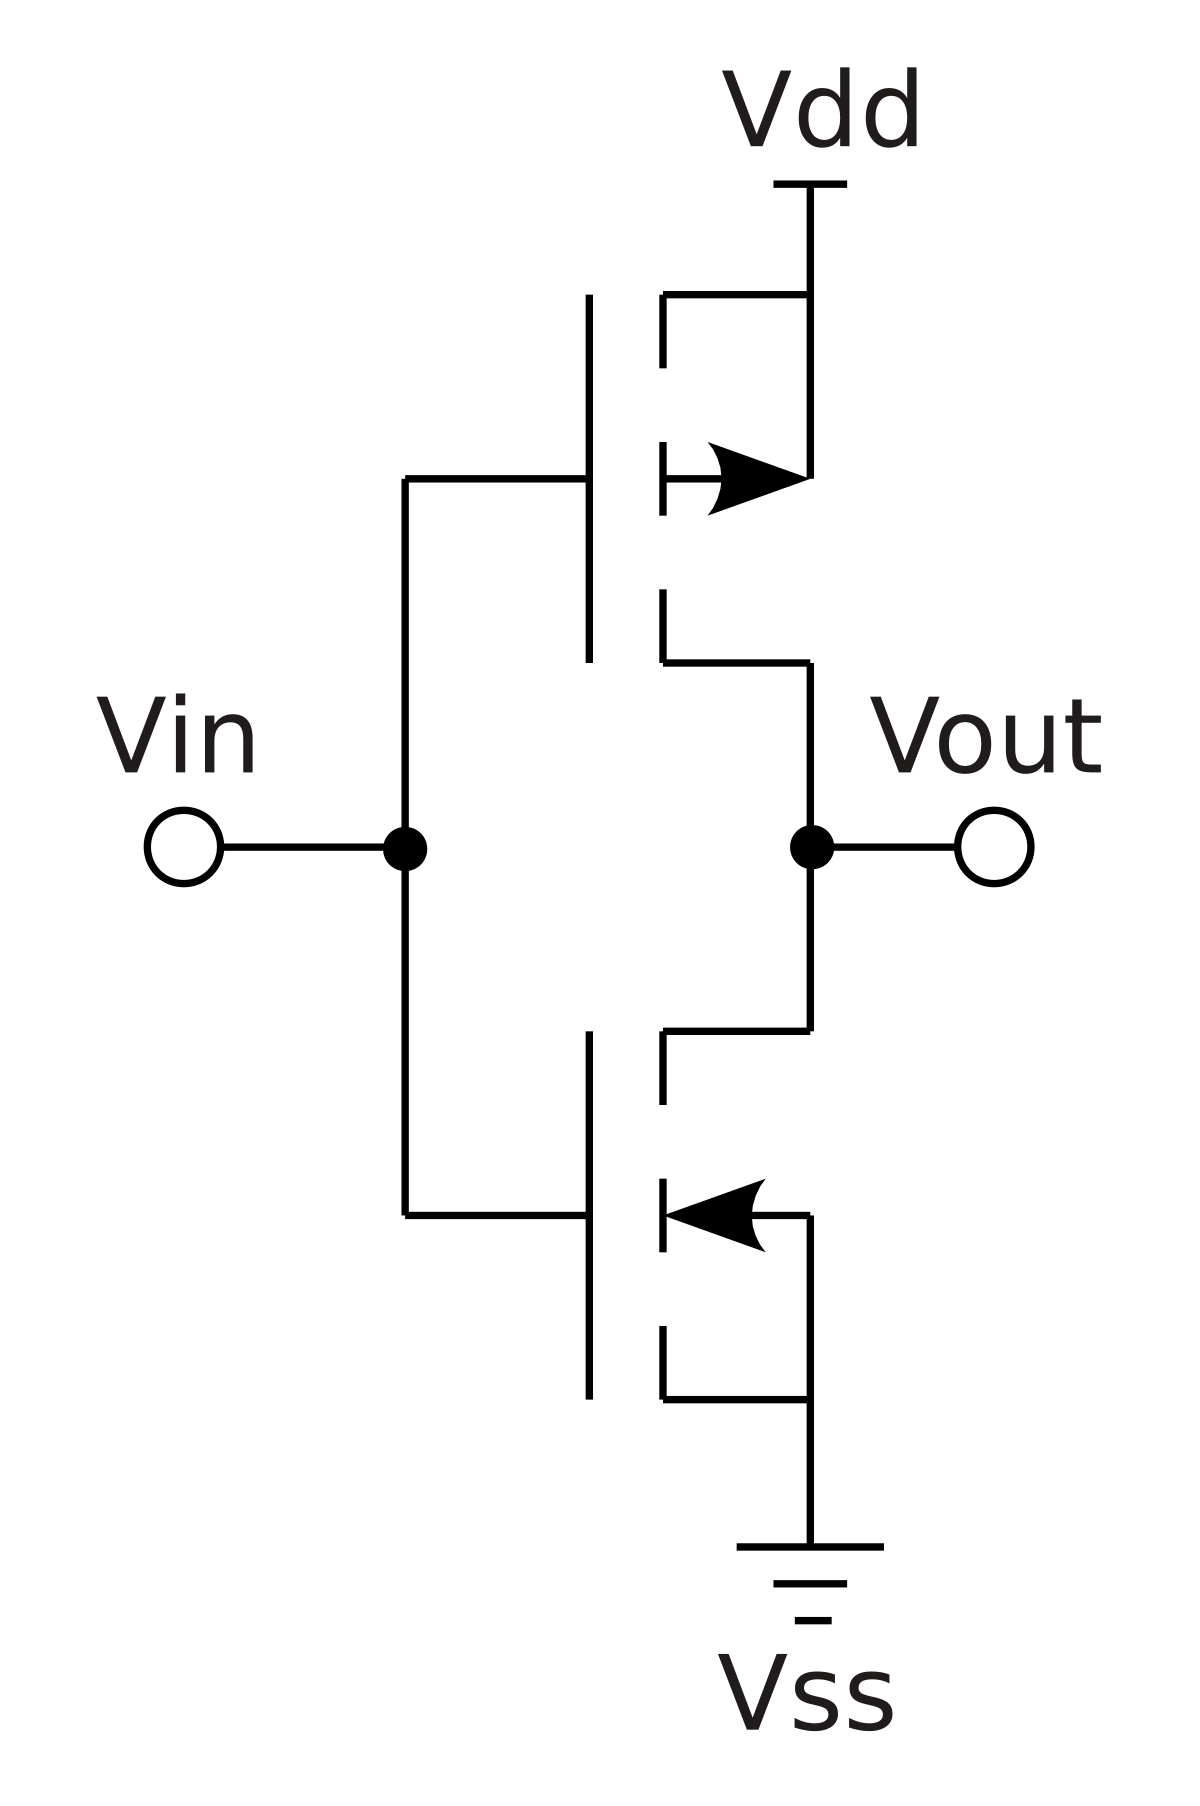
\includegraphics[width=\textwidth]{pictures/CMOS_inverter.png}
            \end{figure}
            \end{center}
        \end{column}
        \begin{column}{0.75\textwidth}
            \begin{center}
                \resizebox{\textwidth}{!}{
                \ctikzset{bipoles/resistor/height=0.1}
                \ctikzset{bipoles/resistor/width=0.3}
                \begin{circuitikz}[american voltages]
                    \draw [thick]
                    (0,0) to [short, *-] (10,0)
                    to [european resistor, l=$Z_L$] (10, 4)
                    (0,0) to [open, v<=$V_S$] (0,4)
                    to [short, *-] (1, 4)
                    to [amp, a=$Z_o \rightarrow 0$] (3, 4)
                    to [short] (6, 4)
                    to [european resistor, l=$Z_0$] (8, 4)
                    to [short] (10,4)
                    ;
                    \draw
                    (0, 0) to [open] (1.25, 4)
                    to [R] (2.75, 4)
                    ;
                \end{circuitikz}
                }
            \end{center}
        \end{column}
    \end{columns}
\end{frame}

\begin{frame}{Matching à la source - Résistance série}
    \begin{columns}
        \begin{column}{0.3\textwidth}
            \begin{itemize}
                \item Ajouter une résistance externe!
                \item Très proche de la sortie
                \bigskip
                \item Valider $Z_o$ du IC
                \item $Z_S = Z_0 - Z_o$
            \end{itemize}
        \end{column}
        \begin{column}{0.7\textwidth}
            \begin{center}
            \resizebox{\textwidth}{!}{
            \ctikzset{bipoles/resistor/height=0.1}
            \ctikzset{bipoles/resistor/width=0.3}
            \begin{circuitikz}[american voltages]
                \draw [thick]
                (0,0) to [short, *-] (10,0)
                to [european resistor, l=$Z_L$] (10, 4)
                (0,0) to [open, v<=$V_S$] (0,4)
                to [short, *-] (1, 4)
                to [amp, a=$Z_o \rightarrow 0$] (3, 4)
                to [european resistor, l=$Z_S$, color=red] (5, 4)
                to [short] (6, 4)
                to [european resistor, l=$Z_0$] (8, 4)
                to [short] (10,4)
                ;
                \draw
                (0, 0) to [open] (1.25, 4)
                to [R] (2.75, 4)
                ;
            \end{circuitikz}
            }
            \end{center}
        \end{column}
    \end{columns}
\end{frame}


\subsection{Matching à la load}

\begin{frame}{Matching à la load}
    \begin{itemize}
        \item Plupart des circuits avec entrée CMOS
        \item $Z_L \rightarrow \infty\Omega$
    \end{itemize}
    \begin{columns}
        \begin{column}{0.25\textwidth}
            \begin{center}
                \begin{figure}
                \centering
                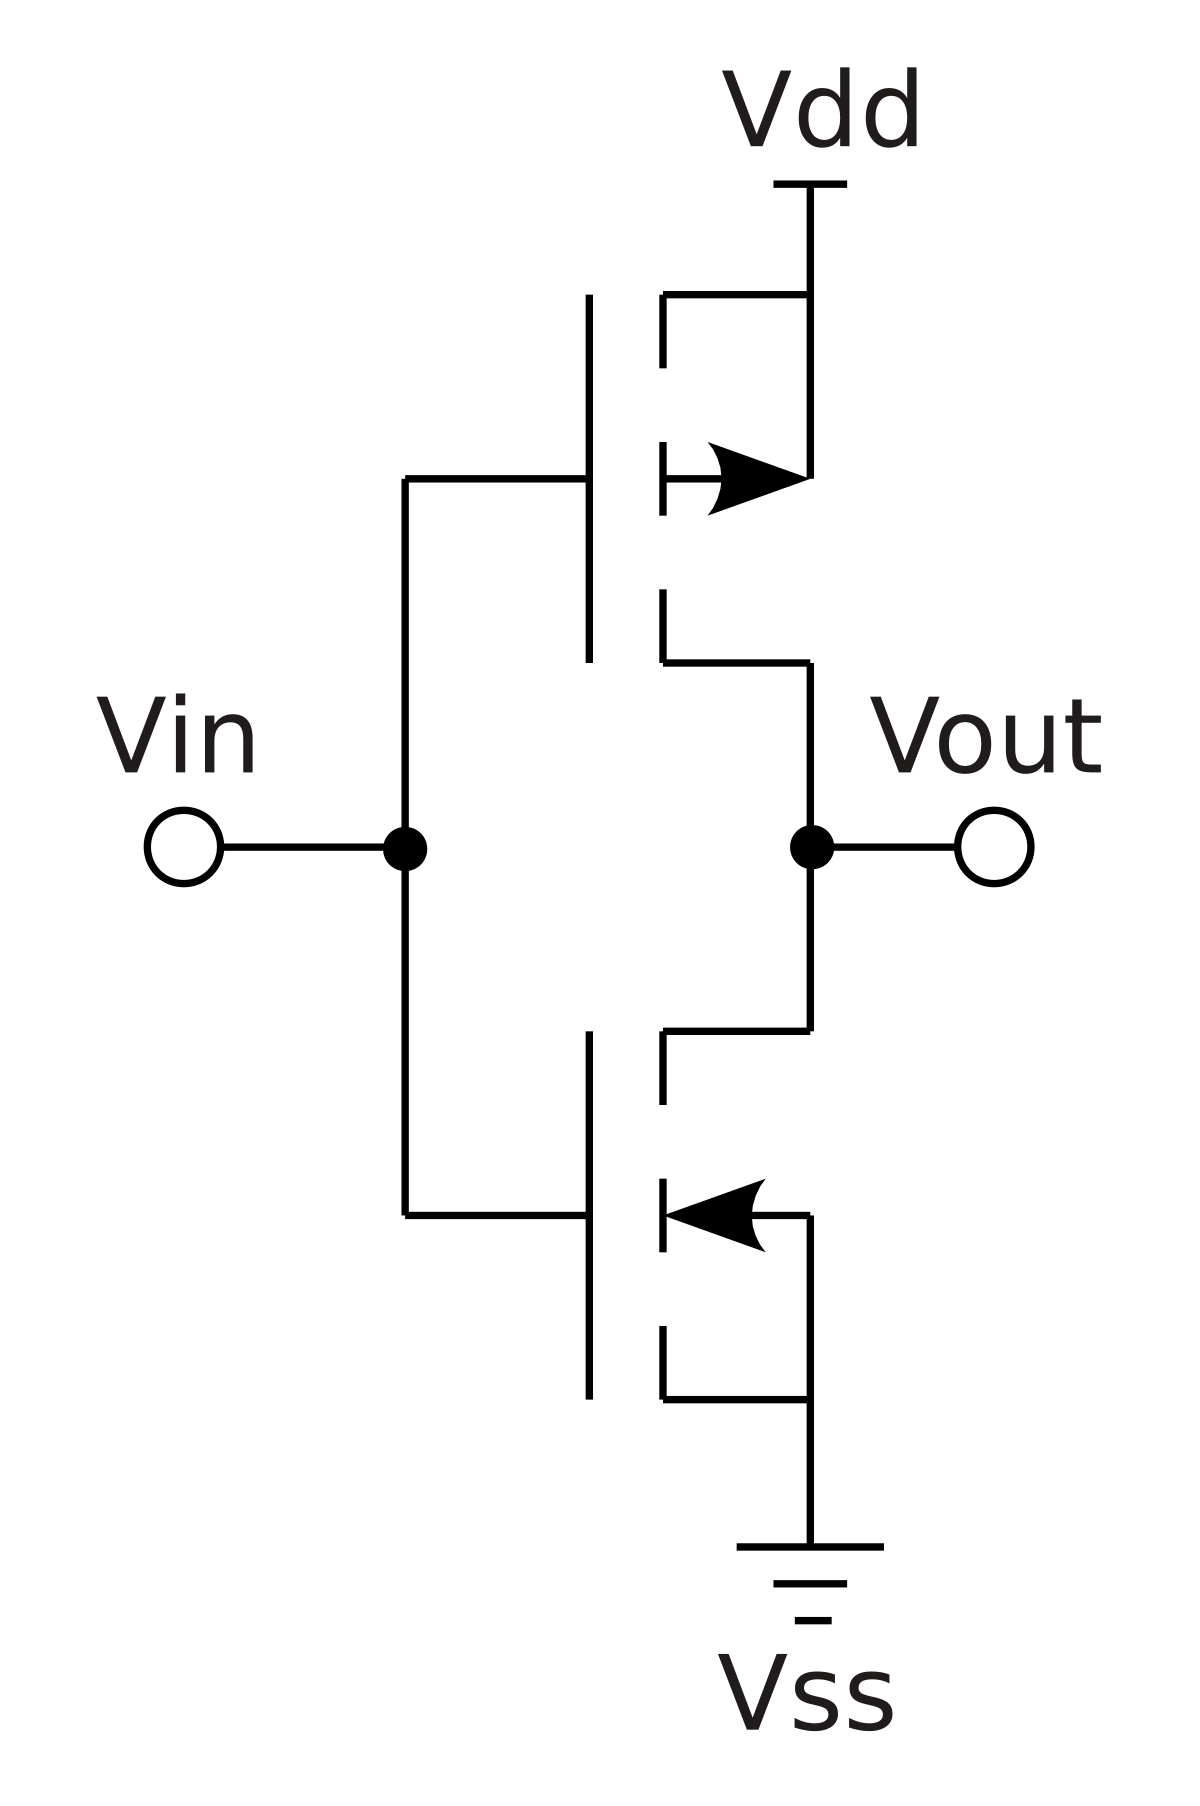
\includegraphics[width=\textwidth]{pictures/CMOS_inverter.png}
            \end{figure}
            \end{center}
        \end{column}
        \begin{column}{0.75\textwidth}
            \begin{center}
                \resizebox{\textwidth}{!}{
                \ctikzset{bipoles/resistor/height=0.1}
                \ctikzset{bipoles/resistor/width=0.3}
                \begin{circuitikz}[american voltages]
                    \draw [thick]
                    (0,0) to [short, *-] (10,0)
                    to [open] (10, 4)
                    (0,0) to [open, v<=$V_S$] (0,4)
                    to [short, *-] (1, 4)
                    to [amp, a=$Z_o \rightarrow 0$] (3, 4)
                    to [european resistor, l=$Z_S$] (4.25, 4)
                    to [european resistor, l=$Z_0$] (7, 4)
                    to [amp, a=$Z_i \rightarrow \infty$] (10, 4)
                    ;
                    \draw
                    (0, 0) to [open] (1.25, 4)
                    to [R] (2.75, 4)
                    ;
                \end{circuitikz}
                }
            \end{center}
        \end{column}
    \end{columns}
\end{frame}

\begin{frame}{Matching à la load - Résistance parallèle}
    \begin{columns}
        \begin{column}{0.3\textwidth}
            \begin{itemize}
                \item Ajouter une résistance externe!
                \item Très proche de l'entrée
                \bigskip
                \item Valider $Z_i$ du IC
                \item $Z_L = Z_0 - \frac{Z_0}{Z_i}$
            \end{itemize}
        \end{column}
        \begin{column}{0.7\textwidth}
            \begin{center}
            \resizebox{\textwidth}{!}{
            \ctikzset{bipoles/resistor/height=0.1}
            \ctikzset{bipoles/resistor/width=0.3}
            \begin{circuitikz}[american voltages]
                \draw [thick]
                    (0,0) to [short, *-] (10,0)
                    to [open] (10, 4)
                    (0,0) to [open, v<=$V_S$] (0,4)
                    to [short, *-] (1, 4)
                    to [amp, a=$Z_o \rightarrow 0$] (3, 4)
                    to [european resistor, l=$Z_S$] (4.25, 4)
                    to [european resistor, l=$Z_0$] (7, 4)
                    to [amp, a=$Z_i \rightarrow \infty$] (10, 4)
                    ;
                \draw [thick]
                    (7.5, 4) to [european resistor, l=$Z_L$, color=red] (7.5, 0)
                    ;
                \draw
                    (0, 0) to [open] (1.25, 4)
                    to [R] (2.75, 4)
                    ;

            \end{circuitikz}
            }
            \end{center}
        \end{column}
    \end{columns}
\end{frame}

\subsection{Matching du conducteur}

\begin{frame}{Impédance caractéristique}
    \begin{itemize}
        \item L'impédance caractéristique $Z_0$ d'une ligne de transmission
        \item Ne dépend que de la \textit{géométrie} de la ligne de transmission
        \item Contrôle les éléments capacitifs et inductifs parasites, qui dominent
        \bigskip
        \item Augmenter largeur de trace $\rightarrow$ plus de capacitance
        \item Augmenter distance entre les traces $\rightarrow$ plus d'inductance
        \bigskip
        \item \textit{Dans un PCB, l'inductance parasite domine toujours!}
    \end{itemize}
\end{frame}

\begin{frame}{Géométries}
    \begin{center}
        \begin{figure}
            \centering
            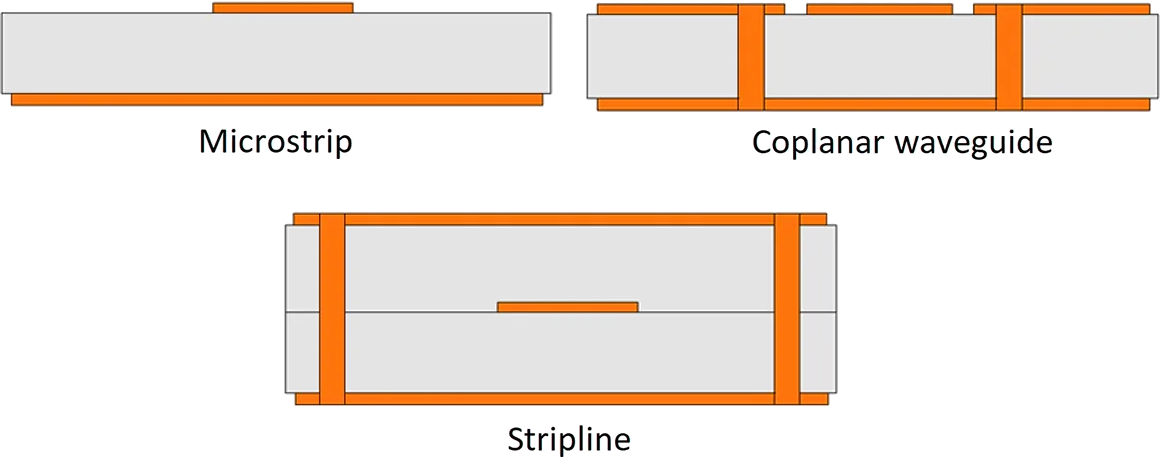
\includegraphics[width=\textwidth]{pictures/microstrip-VS-Stripline-vs-coplanar-waveguide.png}
        \end{figure}
    \end{center}
\end{frame}

\begin{frame}{Microstrip}
    \begin{columns}
        \begin{column}{0.66\textwidth}
            \begin{itemize}
                \item Trace sur le TOP / BOTTOM du PCB
                \item Plan de retour en-dessous de la trace
                \item Diélectrique d'un seul côté
                \item Signal plus rapide
            \end{itemize}
        \end{column}
        \begin{column}{0.33\textwidth}
            \begin{center}
                \begin{figure}
                    \centering
                    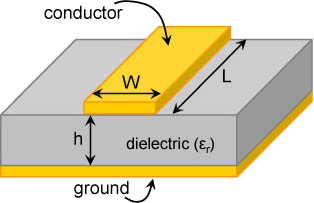
\includegraphics[width=\textwidth]{pictures/microstrip.png}
                \end{figure}
            \end{center}
        \end{column}
    \end{columns}
\end{frame}

\begin{frame}{Microstrip - Formule}
    \begin{itemize}
        \item Norme IPC-2141
        \item Approximation empirique
    \end{itemize}
    \pause
    \begin{center}
        \[
            Z_0 =
            \begin{cases} 
                \dfrac{60}{\sqrt{\varepsilon_{eff}}}\ln\left(8\frac{H}{W} + 0.25\frac{W}{H}\right), & \text{if } \frac{W}{H} < 1 \\
                \dfrac{120 \pi}{\sqrt{\varepsilon_{eff}} \cdot \left(\frac{W}{H} + 1.393 + \frac{2}{3}\ln\left(\frac{w}{H} + 1.444\right)\right)}, & \text{if } \frac{W}{H} \geq 1
            \end{cases}
        \]
        \[
            \varepsilon_{eff} \coloneqq
            \begin{cases} 
                \frac{\varepsilon_r + 1}{2} + \frac{\varepsilon_r - 1}{2} \cdot \left(\left(1 + 12 \frac{H}{W}\right)^{-\frac{1}{2}} + 0.04\left(1 - \frac{W}{H}\right)^2\right), & \text{if } \frac{W}{H} < 1 \\
                \frac{\varepsilon_r + 1}{2} + \frac{\varepsilon_r - 1}{2} \cdot \left(1 + 12 \frac{H}{W}\right)^{-\frac{1}{2}}, & \text{if } \frac{W}{H} \geq 1
            \end{cases}
        \]
    \end{center}
\end{frame}

\subsection{Impédance Différentielle}